\documentclass{article}
\usepackage[T1]{fontenc}
\usepackage{lmodern}
\usepackage{graphicx}
\usepackage{amsmath,amssymb}
\usepackage[a4paper,margin=2cm]{geometry}
\usepackage[absolute,overlay]{textpos}
\setlength{\TPHorizModule}{1mm}
\setlength{\TPVertModule}{1mm}
\usepackage[indonesian]{babel}
\usepackage{hyperref}
\setlength{\emergencystretch}{2em}
% unit: Halaman 13

\begin{document}

% === Halaman 13 (llm) ===

\vspace{237.60mm}

\textcolor{red}{Sumber: H\\u00e5kon Jacobsen, Lecture 2 -- Block ciphers, PRFs/PRPs, DES, AES}

\section*{AES-128}

\vspace{60mm}

% deskripsi: Diagram alur proses enkripsi AES-128 yang menunjukkan proses ekspansi kunci dari kunci utama K menjadi kunci putaran K0 hingga K10, serta struktur 10 putaran yang terdiri dari operasi SubBytes, ShiftRow, dan MixColumn.
% bbox normalisasi: [0.0150, 0.1400, 0.9850, 0.9400]
\begin{textblock*}{203.70mm}(3.15mm,41.58mm)
\noindent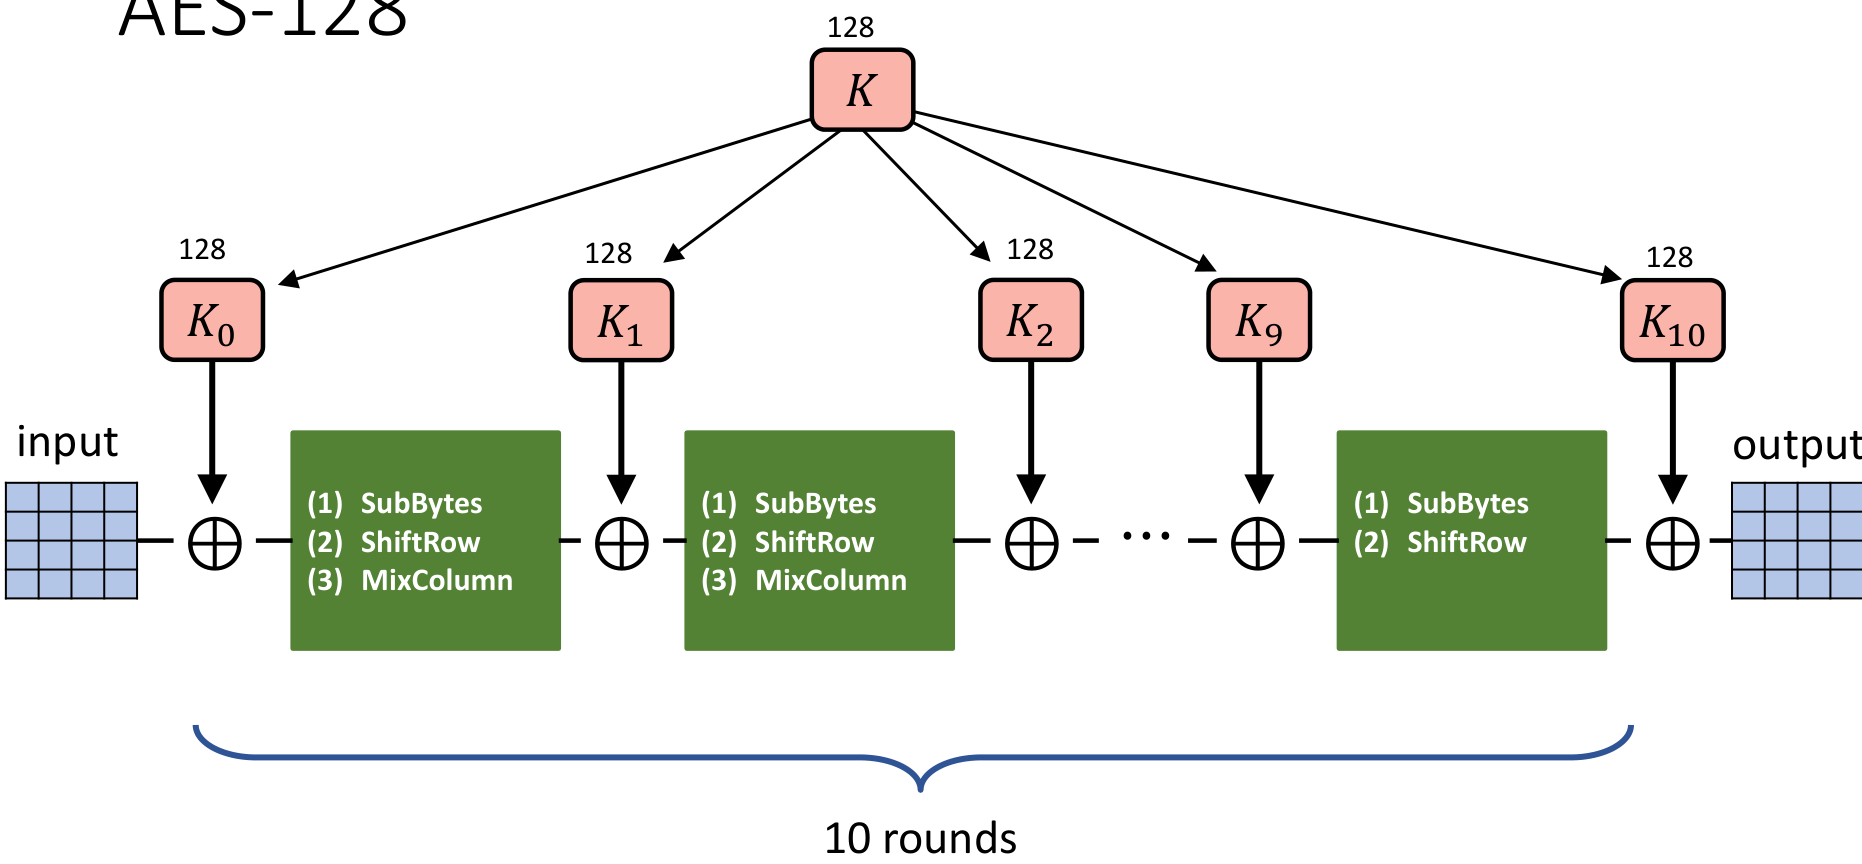
\includegraphics[width=203.70mm,height=237.60mm]{../../images/llm/page_013_img_01.png}%
\end{textblock*}

\end{document}
